% -*- latex -*-
%%%%%%%%%%%%%%%%%%%%%%%%%%%%%%%%%%%%%%%%%%%%%%%%%%%%%%%%%%%%%%%%
%%%%
%%%% This TeX file is part of the course
%%%% Introduction to Scientific Programming in C++/Fortran2003
%%%% copyright 2017-2022 Victor Eijkhout eijkhout@tacc.utexas.edu
%%%%
%%%% warmup.tex : chapter of preliminary stuff
%%%%
%%%%%%%%%%%%%%%%%%%%%%%%%%%%%%%%%%%%%%%%%%%%%%%%%%%%%%%%%%%%%%%%

\Level 0 {Programming and computational thinking}

In this chapter we take a look at the history of computers and computer programming,
and think a little about what programming involves.

\begin{slide}{Earliest computers}
  \label{sl:neumann}
  Historically, computers were used for big physics calculations, for
  instance, atom bomb calculations\\

  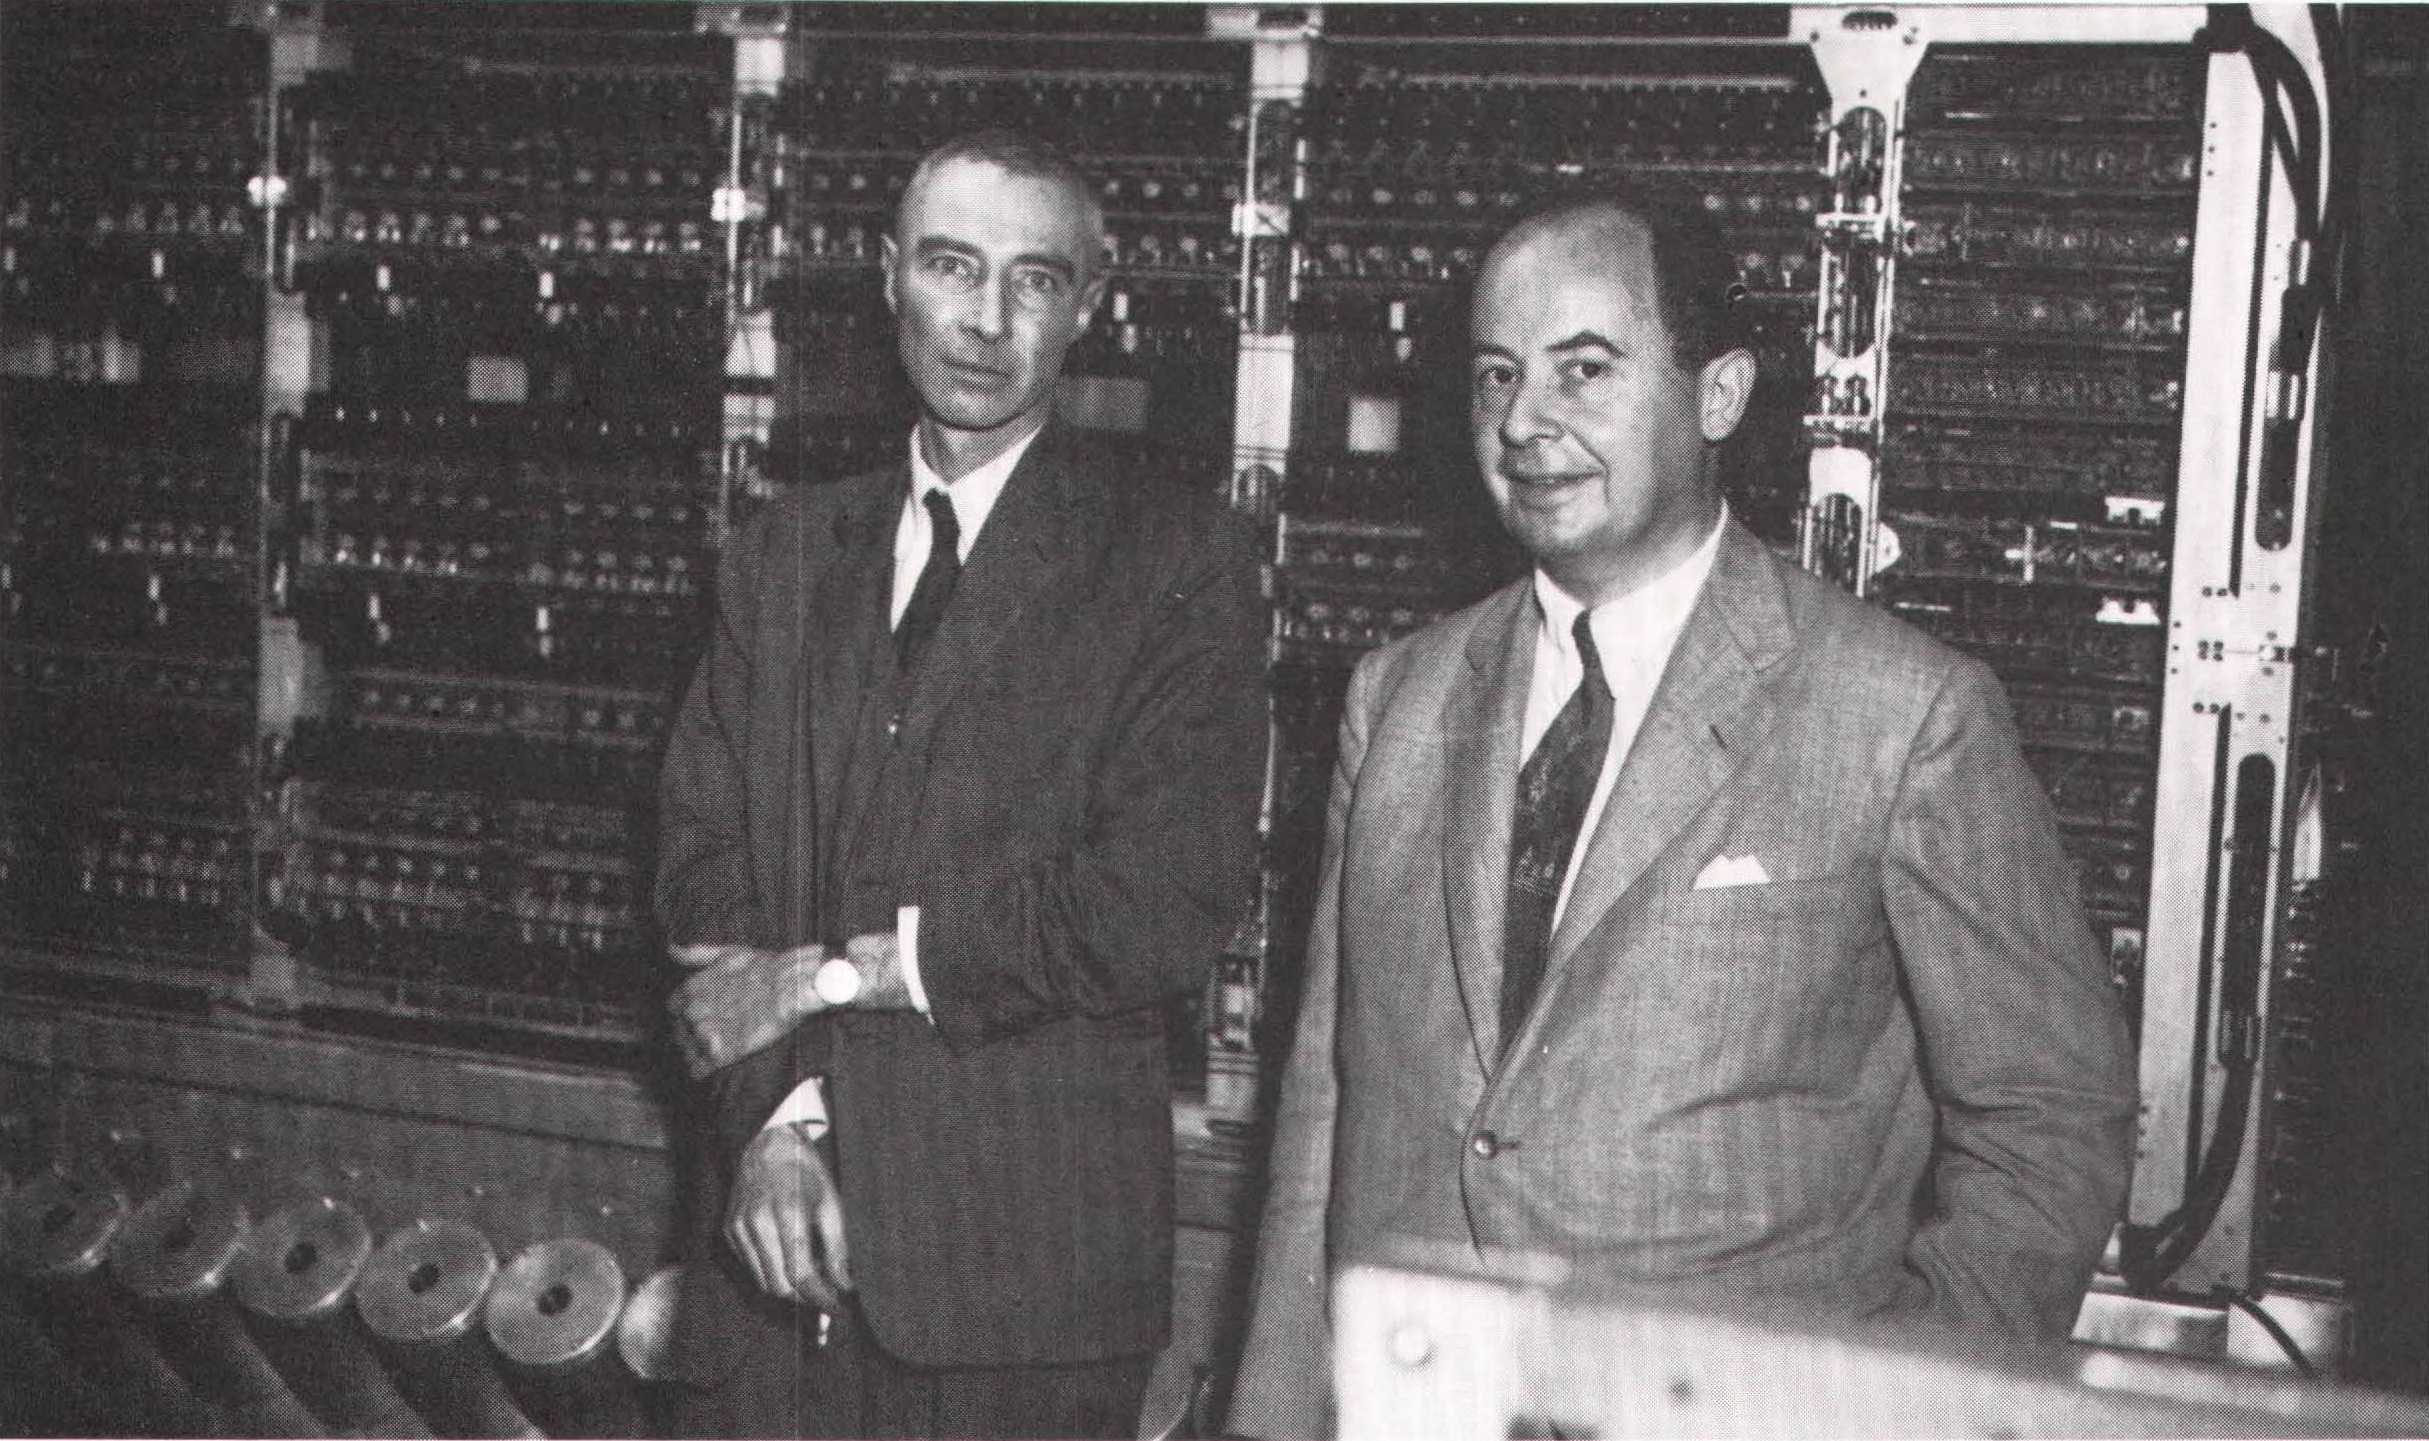
\includegraphics[scale=.5]{neumann}

  (Robert Oppenheimer and John von Neumann)
\end{slide}

\begin{slide}{Hands-on programming}
  \label{sl:eniac}
  Very early computers such as ENIAC were hardwired\\
  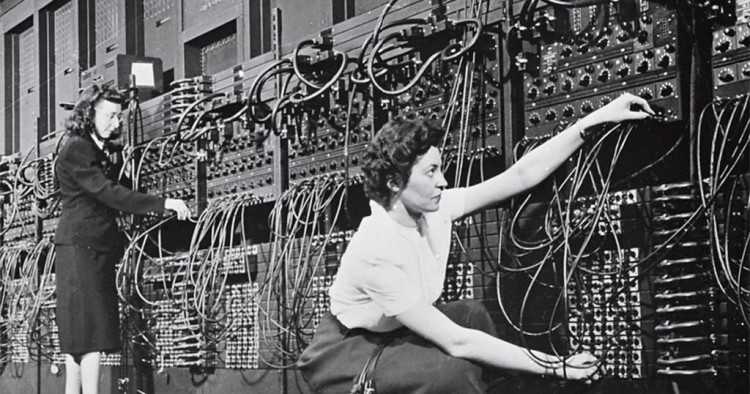
\includegraphics[scale=.4]{eniac-programming}\\
  later became `stored program' computer.\\
  see \url{http://eniacprogrammers.org/}
\end{slide}

\begin{slide}{Program entry}
  \label{sl:punch}
  Later programs were written on punchcards\\
  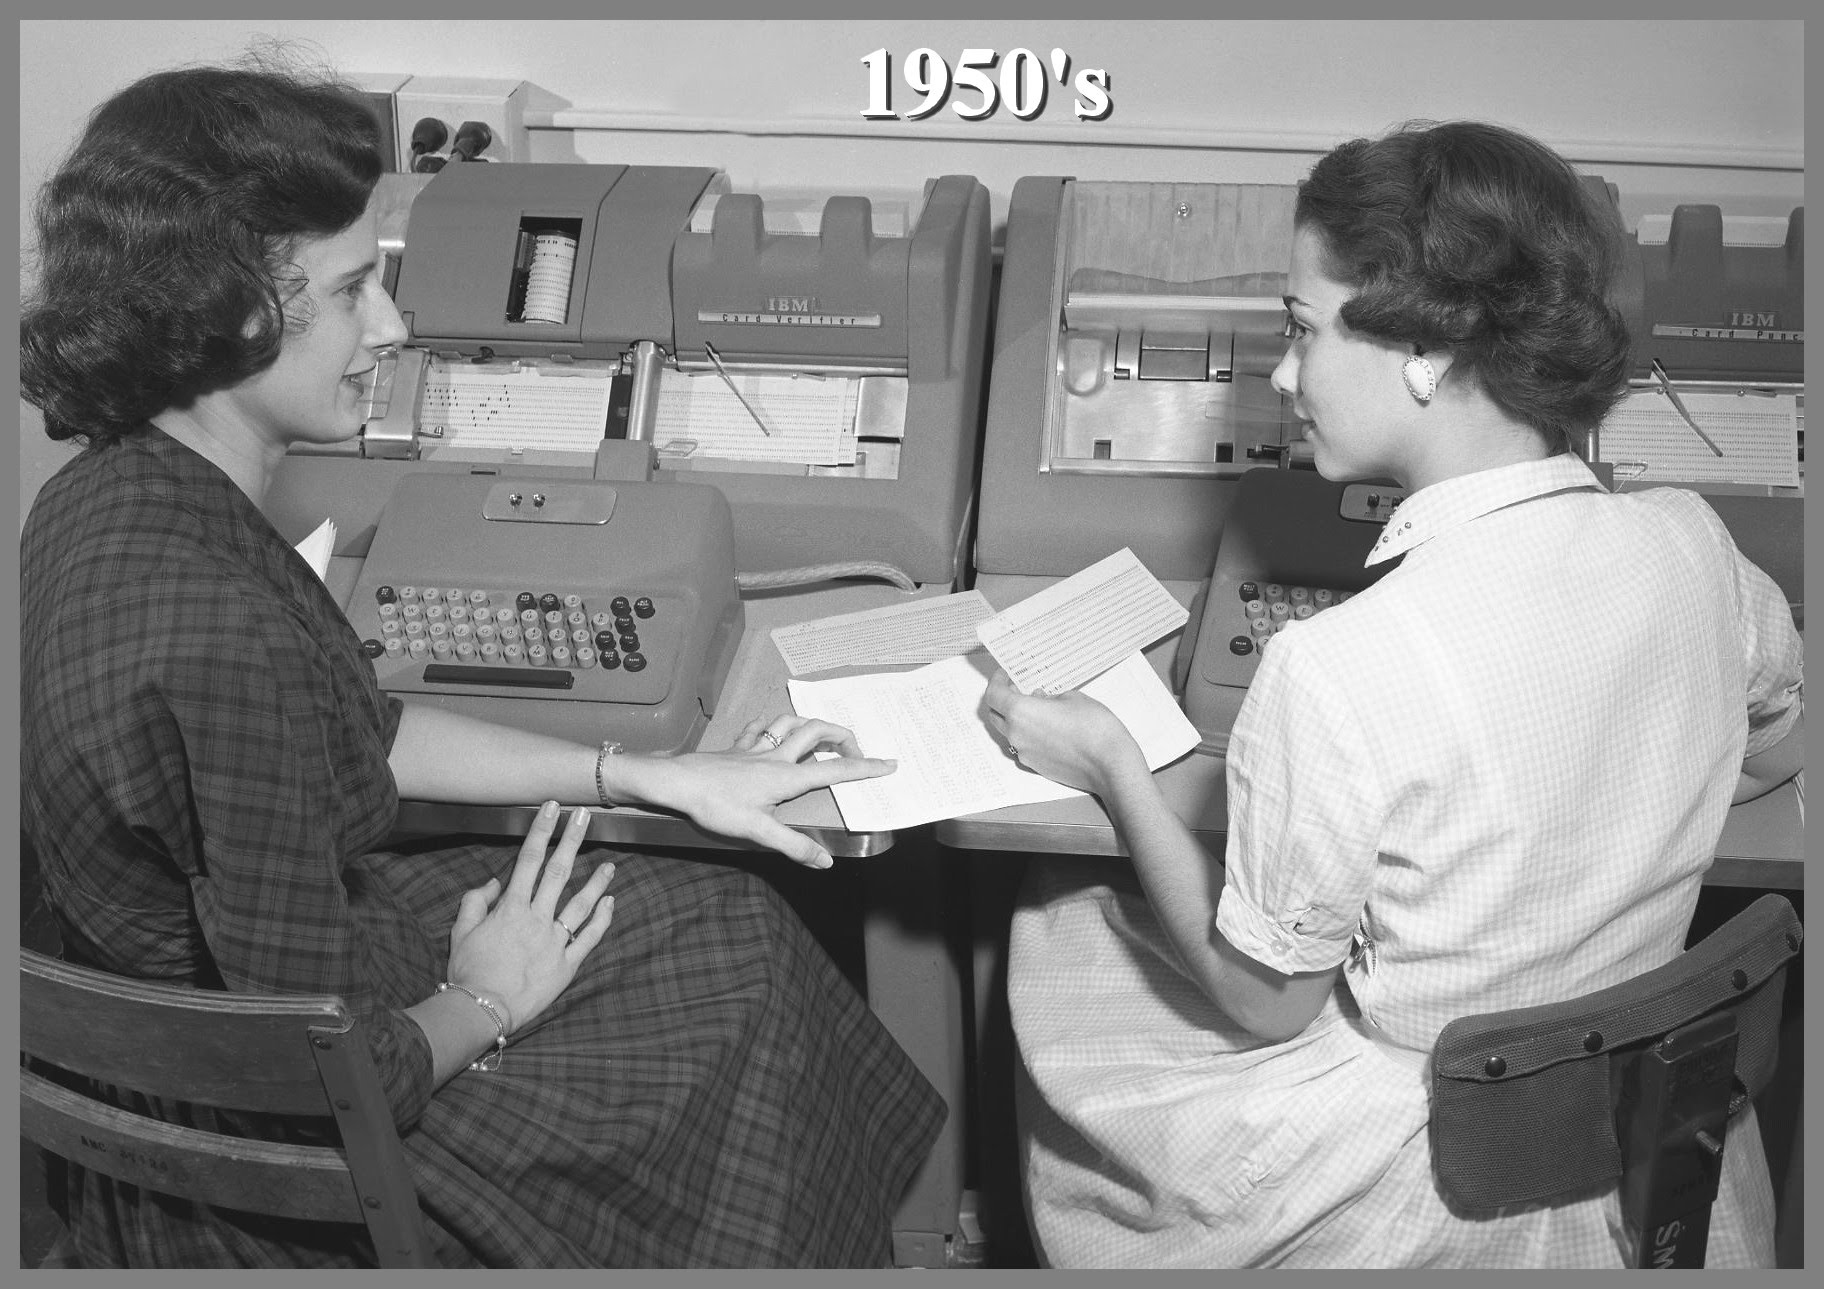
\includegraphics[scale=.14]{punchcards}
\end{slide}

\begin{slide}{The first programming language}
  \label{sl:fcard}
  Initial programming was about translating the math formulas; after a
  while they made a language for that: FORmula TRANslation\\
  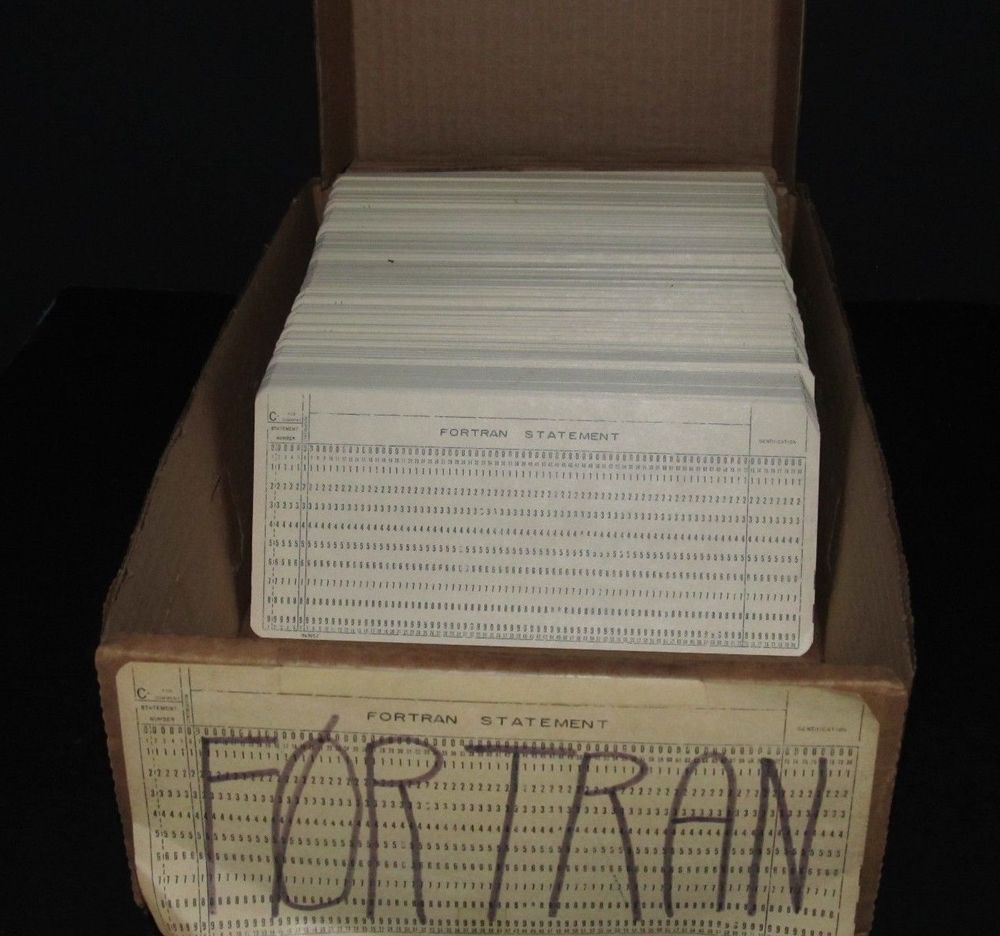
\includegraphics[scale=.2]{fortrancards}
\end{slide}

\begin{slide}{Programming is everywhere}
  \label{sl:progeverywhere}
  Programming is used in many different ways these days.
  \begin{itemize}
  \item You can make your own commands in
    \indextermbus{Microsoft}{Word}.
  \item You can make apps for your \indexterm{smartphone}.
  \item You can solve the riddles of the universe using big computers.
  \end{itemize}
  This course is aimed at people in the last category.
\end{slide}

\Level 1 {History}

In the early days of computing, hardware design was seen as
challenging, while programming was little more than data entry.
\begin{figure}[ht]
  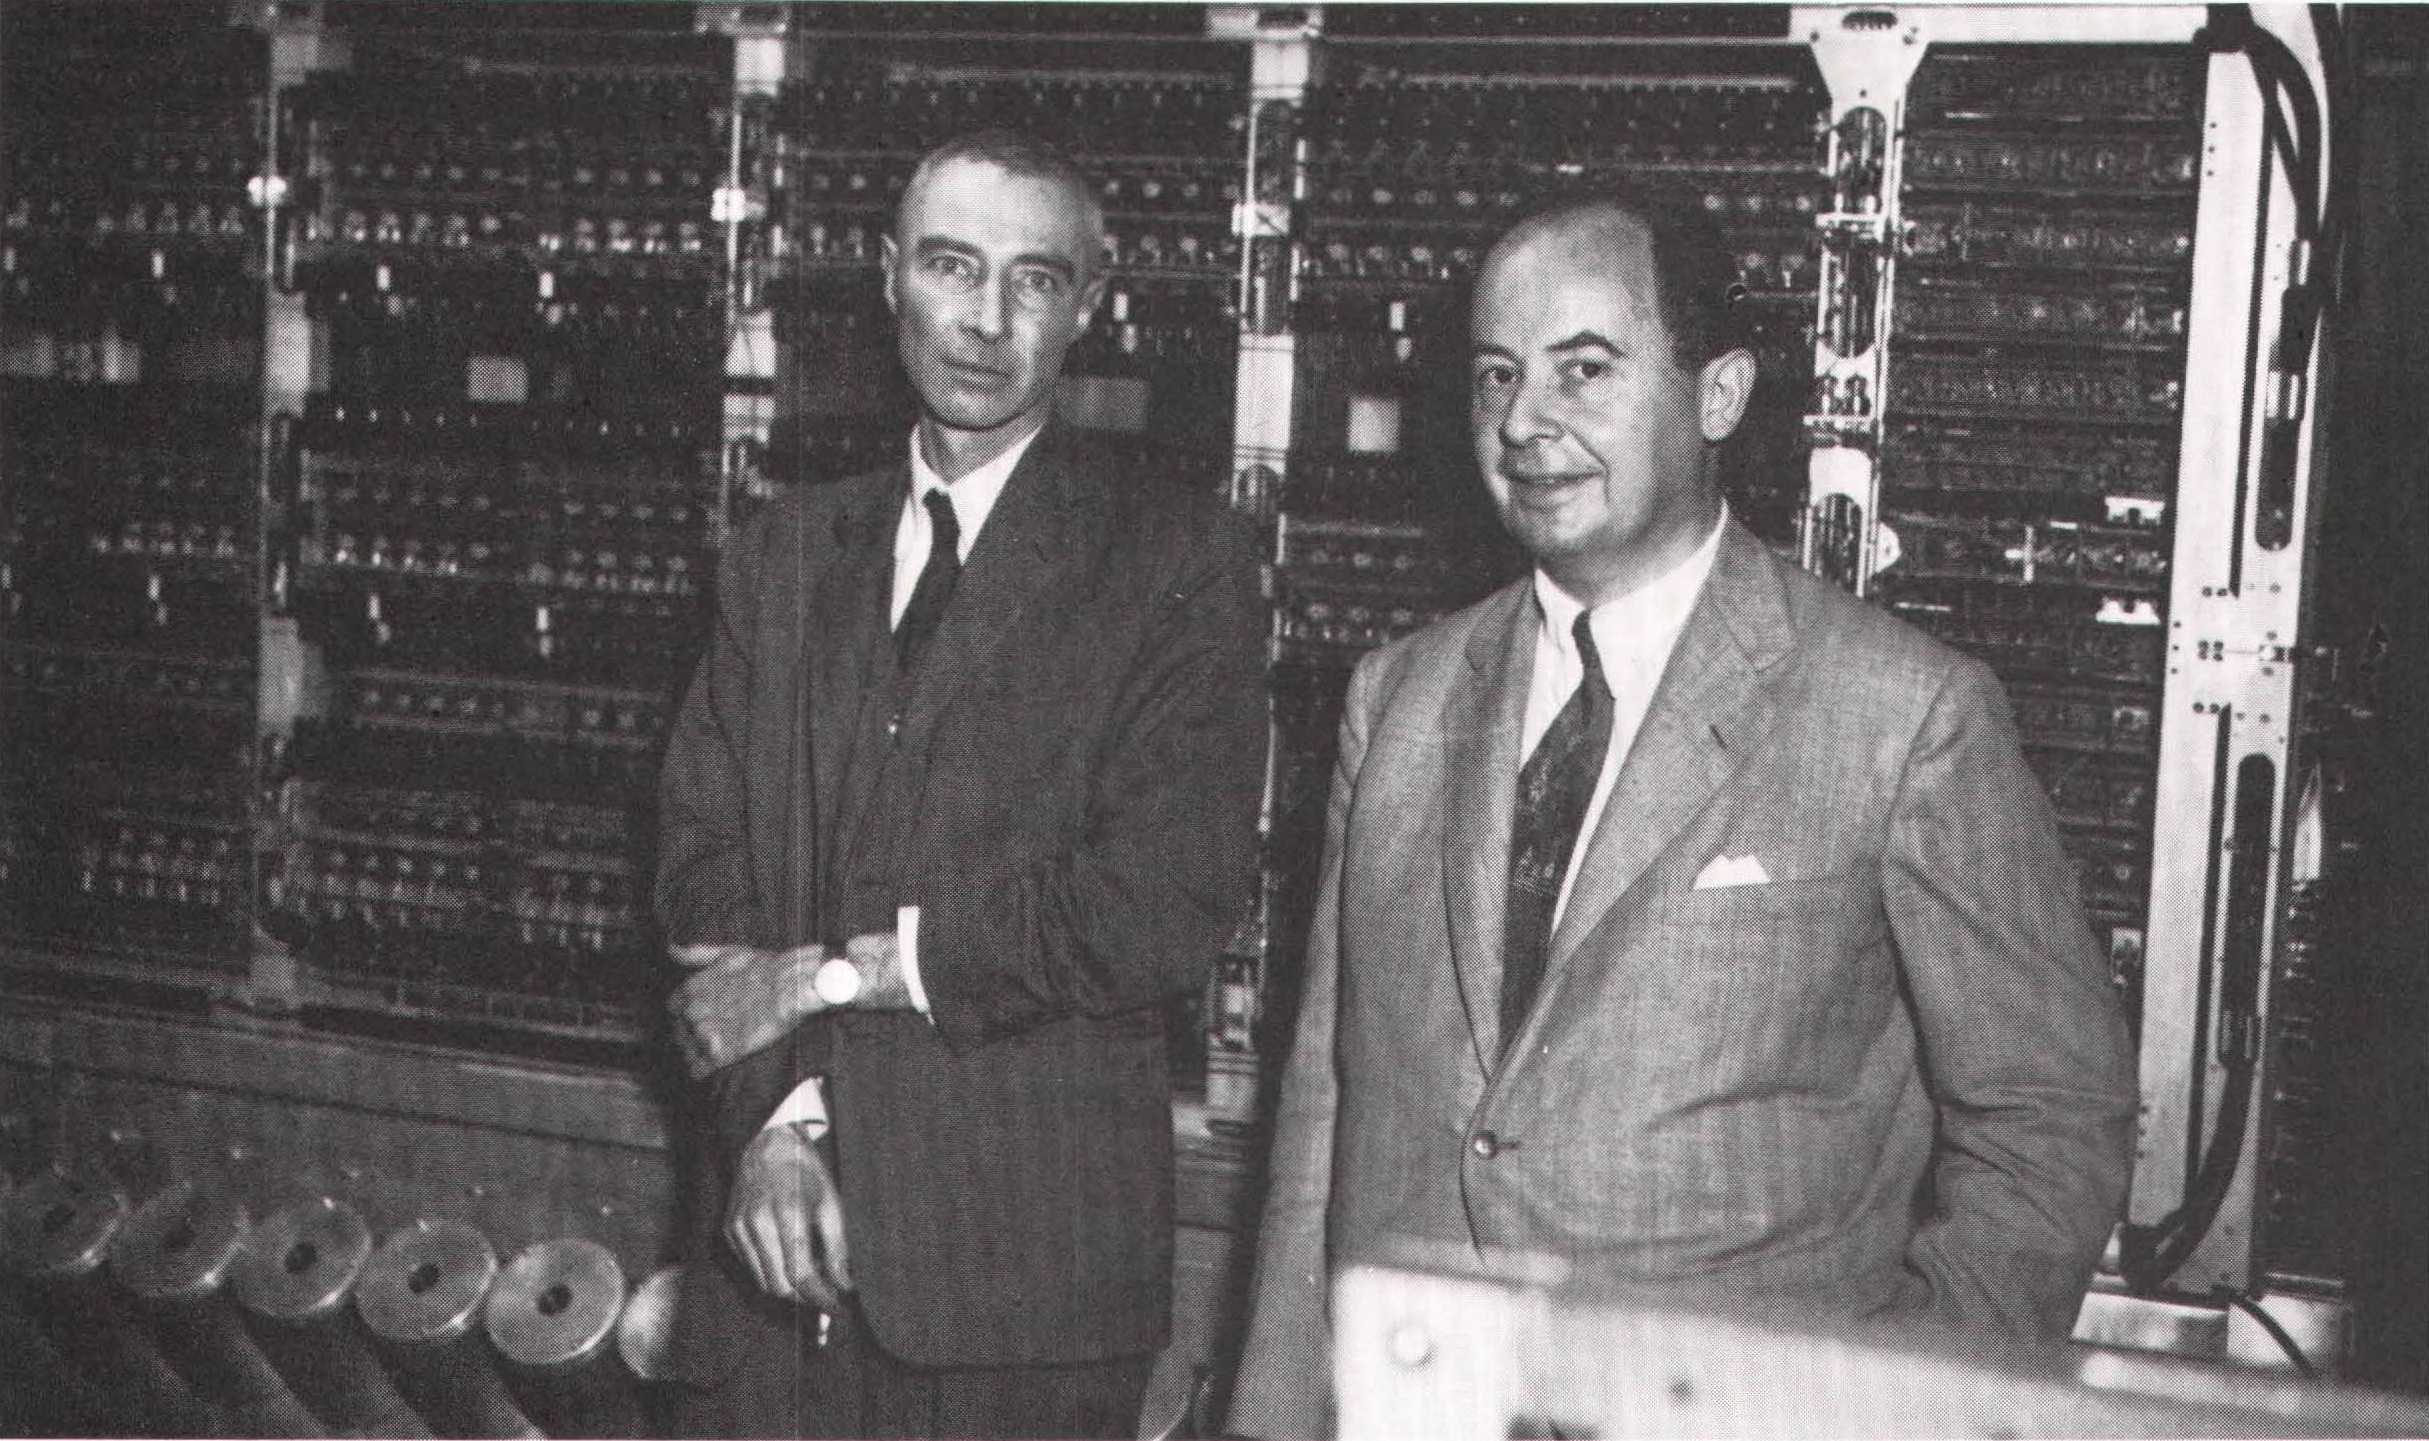
\includegraphics[scale=.5]{neumann}
  \caption{Robert Oppenheimer and John von Neumann}
\end{figure}
The fact that one of the earliest programming languages was called `Fortran',
for  `formula translation', speaks to this:
once you have the math, programming was thought to be nothing more than translating
the math into code. The fact that programs could have subtle errors,
or \emph{bugs}\index{bug}, came as quite a surprise
to the earliest computer designers.

The fact that programming was not as highly valued also had the
side-effect that many of the early programmers were women.
\begin{figure}[ht]
  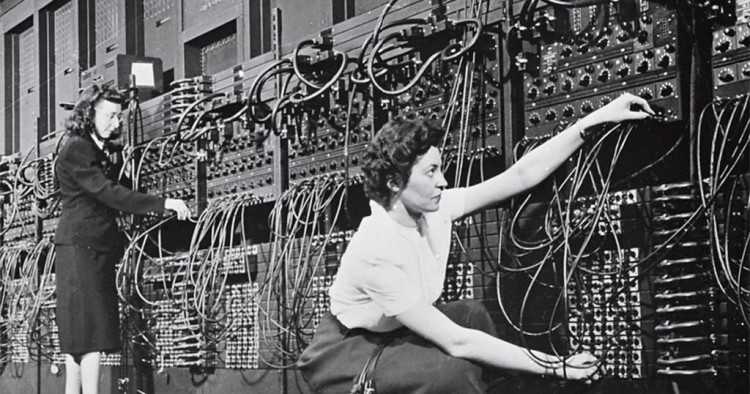
\includegraphics[scale=.4]{eniac-programming}\\
  \caption{Programming the ENIAC}
\end{figure}
Before electronic computers, a `computer' was a person executing
computations, probably with a mechanical calculating device,
and often these were women. From this, the earliest people
programming electronic computers to perform these calculations were,
usually mathematically educated, women.
Two famous
examples were Navy Rear-admiral Grace Hopper, inventor of the Cobol
language, and Margaret Hamilton who led the development of the Apollo
\begin{figure}[ht]
  \begin{multicols}{2}
    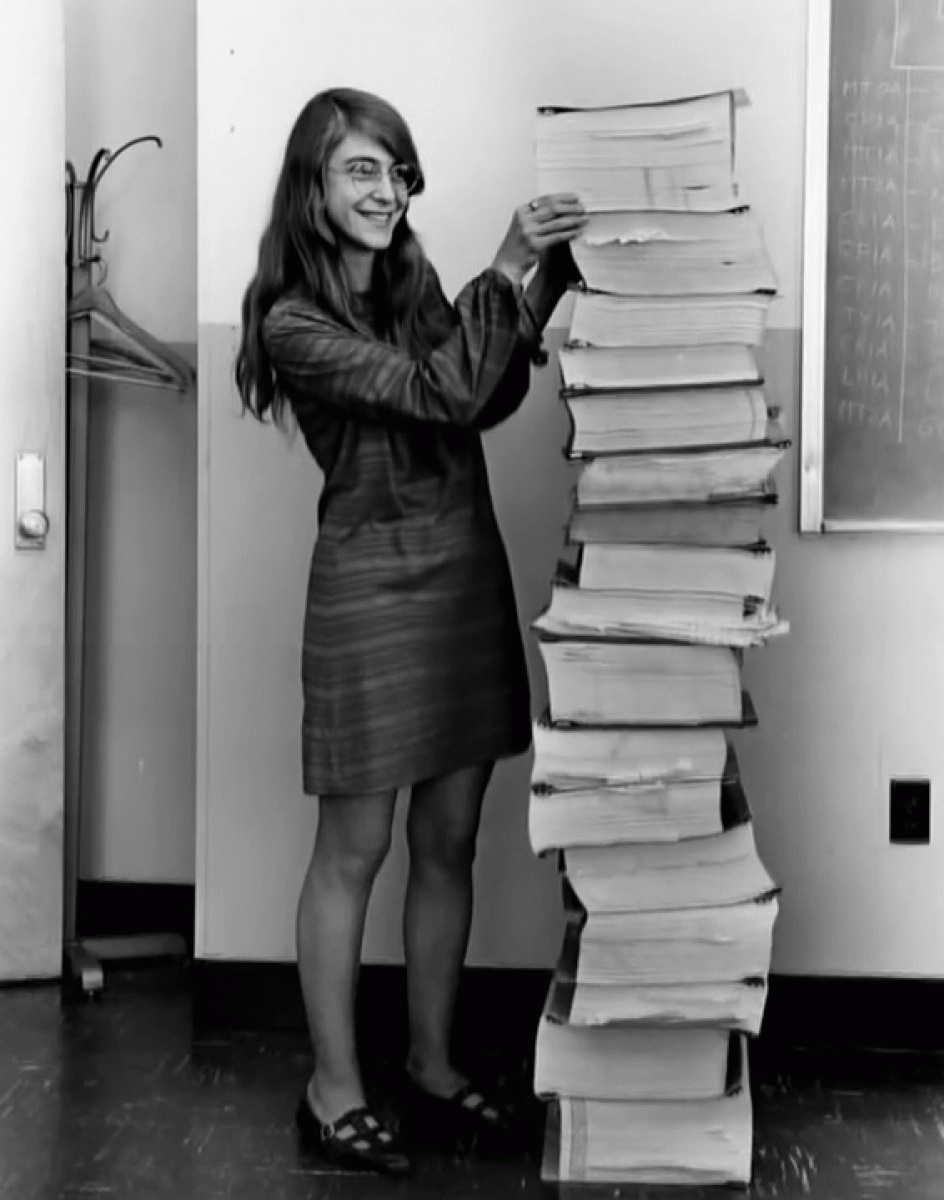
\includegraphics[scale=.09]{hamilton}
    \vfill\columnbreak
    \textsl
    {\small Margaret Hamilton, director of the Software Engineering Division,
    the MIT Instrumentation Laboratory, which developed on-board
    software for the Apollo program.}\par
    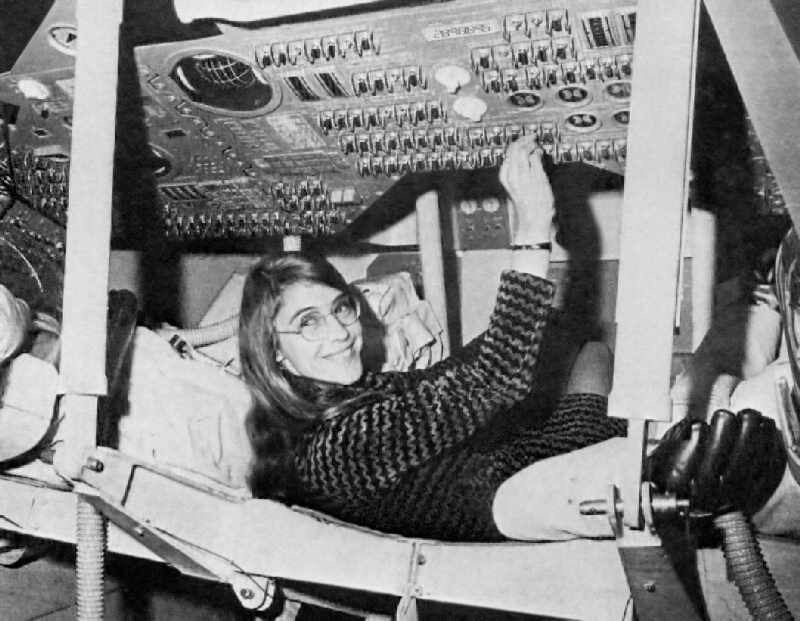
\includegraphics[scale=.10]{Margaret_Hamilton_in_action}
    \vfill\hbox{}\columnbreak
    \caption{Margaret Hamilton}
  \end{multicols}
\end{figure}
program software. This situation changed after the 1960s and certainly
with the advent of
PCs\footnote{\url{http://www.sysgen.com.ph/articles/why-women-stopped-coding/27216}}.

\Level 1 {Is programming science, art, or craft?}

As the previous section argued, programming is more than simple
translation of math into instructions for hardware.
Could it be a science?
There are certainly scientific aspects to programming:
\begin{itemize}
\item Algorithms and complexity theory have a lot of math in them.
\item Programming language design is another mathematically tinged subject.
\end{itemize}
However, programming itself is not a science.

The term `software engineering' may lead you to suspect
that designing and producing software is an engineering discpline,
but this is also not quite the case.
There is no certification for software engineers, and
there is no body of accepted techniques the way there is
for civil engineering and such discplines.

For a large part programming is a discipline. What constitutes a
good program is a matter of taste. That does not mean that there
aren't recommended practices. In this course we will emphasize certain
practices that we think lead to good code, as likewise will discourage
you from certain idioms.

None of this is an exact science. There are multiple programs that
give the right output. However, programs are rarely static. They often
need to be amended or extended, or even fixed, if erroneous behaviour
comes to light, and in that case a badly written program can be a
detriment to programmer productivity. An important consideration,
therefore, is intelligibility of the program, to another programmer,
to your professor in this course, or even to yourself two weeks from
now.

\begin{slide}{Is programming a craft or a science?}
  \label{sl:programmingcraft}
  How about a `discipline'?
\end{slide}

\Level 1 {Computational thinking}

\begin{slide}{Programming is not simple}
  \label{sl:hamilton}
  \small
  Programs can get pretty big:

  \begin{multicols}{2}
    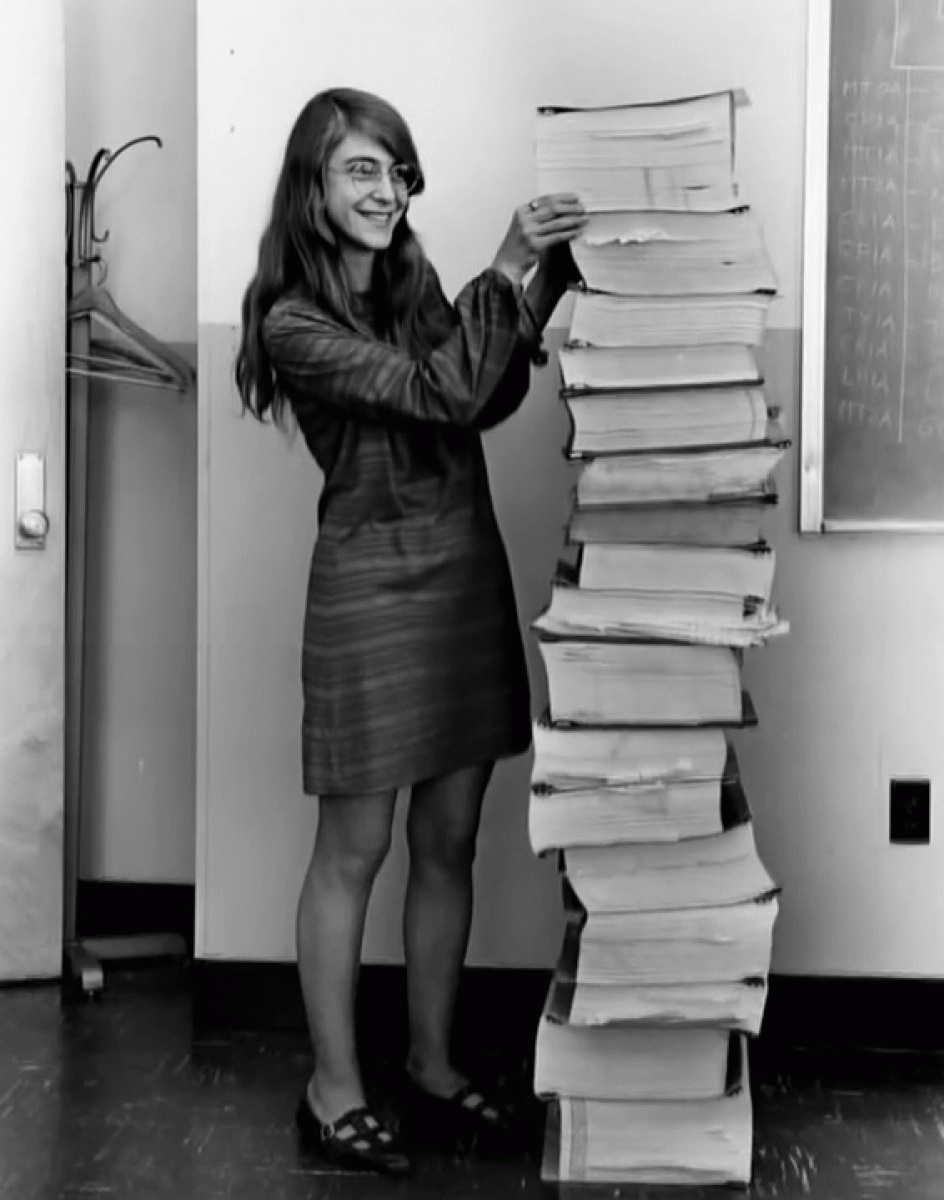
\includegraphics[scale=.09]{hamilton}
    \vfill\columnbreak
    \textsl
    {\small Margaret Hamilton, director of the Software Engineering Division,
    the MIT Instrumentation Laboratory, which developed on-board
    software for the Apollo program.}\par
    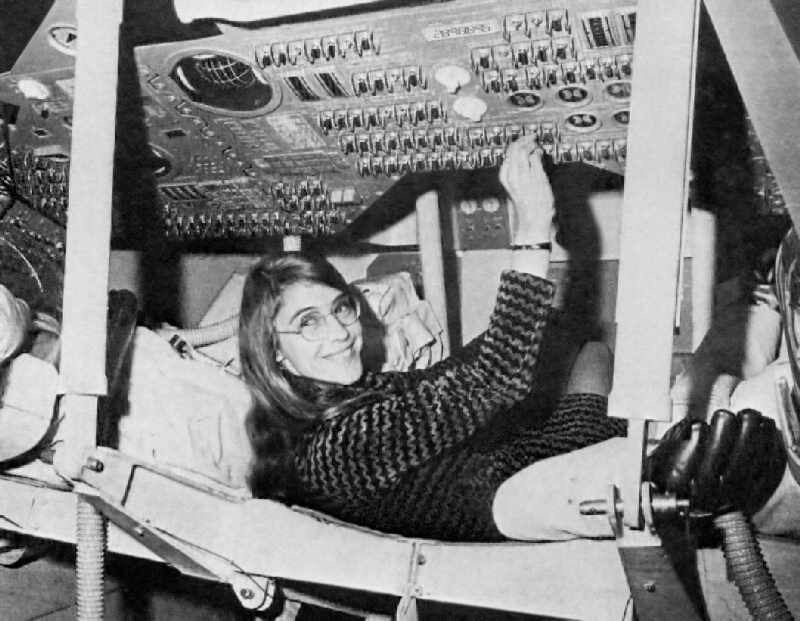
\includegraphics[scale=.10]{Margaret_Hamilton_in_action}
    \vfill\hbox{}\columnbreak
  \end{multicols}

  \framebox{\vbox{\noindent It's not just translating formulas anymore.\par
      Translating ideas to computer code: computational thinking.}
  }

  %% \setbox0=\hbox{%
  %% \begin{parbox}{.8\hsize}
  %% \end{parbox}
  %% }
  %% \begin{framebox}{\box0}    
  %% \end{framebox}

\end{slide}

\begin{block}{Computational thinking: elevator scheduling}
  \label{sl:elevator}
  Mathematical thinking:
  \begin{itemize}
  \item Number of people per day, speed of elevator $\Rightarrow$ yes,
    it is possible to get everyone to the right floor.
  \item Distribution of people arriving \emph{etc.} $\Rightarrow$
    average wait time.
  \end{itemize}
  Sufficient condition $\not=$ existence proof.

  Computational thinking: actual design of a solution
  \begin{itemize}
  \item Elevator scheduling: someone at ground level presses the
    button, there are cars on floors 5 and~10; which one do you send down?
  \end{itemize}
  Coming up with a strategy takes creativity!
\end{block}

\begin{exercise}
  \label{ex:hair}
  A straightforward calculation is the simplest example of an
  algorithm.

  Calculate how many schools for hair dressers the US can
  sustain. Identify the relevant factors, estimate their sizes, and
  perform the calculation.
\end{exercise}

\begin{exercise}
  \label{ex:googlecar}
  Algorithms are usually not uniquely determined:\\
  there is more than one way solve a problem.

  Four self-driving cars arrive simultaneously at an all-way-stop intersection. Come
  up with an algorithm that a car can follow to safely cross the
  intersection. If you can come up with more than one algorithm, what
  happens when two cars using different algorithms meet each other?
\end{exercise}

\begin{block}{Computation and complexity}
  \label{sl:phonebook}
  Looking up a name in the phone book
  \begin{itemize}
  \item start on page~1, then try page~2, et cetera
  \item or start in the middle, continue with one of the halves.
  \end{itemize}
  What is the average search time in the two cases?

  Having a  correct solution is not enough!
\end{block}

\begin{block}{Programming languages are about ideas}
  \label{sl:sussman}
  \begin{quotation}
    \raggedright\noindent
    A powerful programming language serves as a framework within which
    we organize our ideas. Every programming language has three
    mechanisms for accomplishing this:
    \begin{itemize}
    \item primitive expressions
    \item means of combination
    \item means of abstraction
    \end{itemize}
    \textsl{Abelson and Sussman, The Structure and Interpretation of
      Computer Programs}
  \end{quotation}
\end{block}

\begin{block}{Abstraction}
  \label{sl:abstraction}
  \begin{itemize}
  \item The elevator programmer probably thinks: `if the button is
    pressed', not `if the voltage on that wire is 5~Volt'.
  \item The Google car programmer probably writes: `if the car before me
    slows down', not `if I see the image of the car growing'.
  \item \ldots~but probably another programmer had to write that translation.
  \end{itemize}
  A program has layers of abstractions.
\end{block}

\begin{block}{Abstraction is good}
  \label{sl:abstraction-good}
  Abstraction means your program talks about your application
  concepts, rather than about numbers and characters and such.

  Your program should read like a story about your application; not
  about bits and bytes.

  Good programming style makes code intelligible and maintainable.

  (Bad programming style may lead to lower grade.)
\end{block}

\begin{block}{Trust him, he's Dutch!}
  \label{sl:dijkstra-trick}
  \begin{quotation}
    \raggedright\noindent
    The competent programmer is fully aware of the strictly limited
    size of his own skull; therefore he approaches the programming
    task in full humility, and among other things he avoids clever
    tricks like the plague ---~Edsger~Dijkstra
  \end{quotation}  
\end{block}

\begin{block}{Data abstraction}
  \label{sl:stackabstract}
  What is the structure of the data in your program?

  \begin{multicols}{2}
    Stack: you can only get at the top item\\

    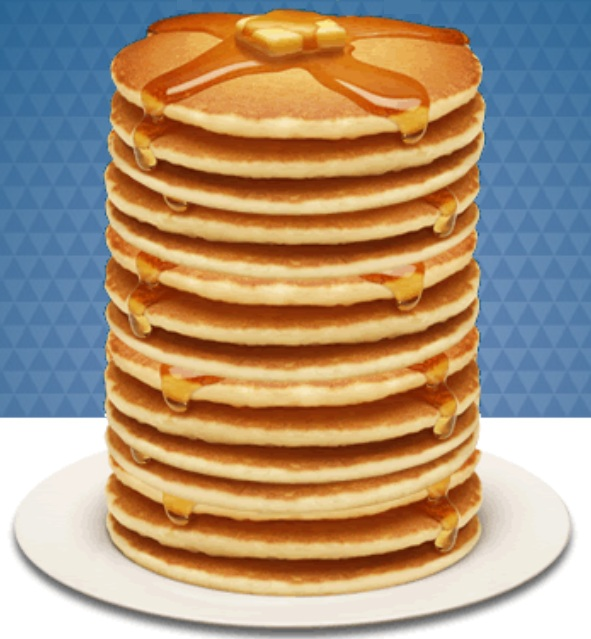
\includegraphics[scale=.22]{stack}
    \vfill\columnbreak
    Queue: items get added in the back, processed at the front\\

    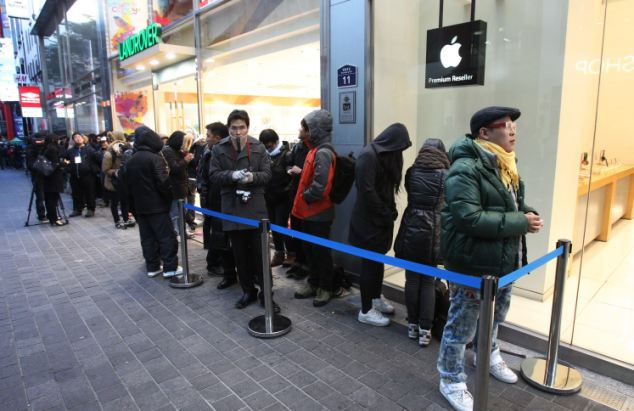
\includegraphics[scale=.22]{queue}
  \end{multicols}
  A program contains structures that support the algorithm. You may
  have to design them yourself.
\end{block}

\Level 1 {Hardware}

\begin{block}{Do you have to know much about hardware?}
  \label{sl:hardwarevid}
  Yes, it's there, but we don't think too much about it in this course.

  Advanced programmers know that hardware influences the speed of
  execution (see TACC's ISTC course).
\end{block}

\Level 1 {Algorithms}

\begin{block}{What is an algorithm?}
  \label{sl:whatalgo}
  \begin{quotation}
    \raggedright\noindent
    An algorithm is a sequence of unambiguous instructions for solving
    a problem, i.e., for obtaining a required output for any
    legitimate input in a finite amount of time\\\relax [A. Levitin,
      Introduction to The Design and Analysis of Algorithms,
      Addison-Wesley, 2003]
  \end{quotation}
  The instructions are written in some language:
  \begin{itemize}
  \item We will teach you C++ and Fortran;
  \item the compiler translates those languages to machine language
  \end{itemize}
\end{block}

\begin{block}{Program steps}
  \label{sl:step-by-step}
  \begin{itemize}
  \item Simple instructions: arithmetic.
  \item Complicated instructions: control structures
    \begin{itemize}
    \item conditionals
    \item loops
    \end{itemize}
  \end{itemize}
\end{block}

\begin{block}{Program data}
  \label{sl:prog-data}
  \begin{itemize}
  \item Input and output data: to/from file, user input, screen
    output, graphics.
  \item Data during the program run:
    \begin{itemize}
    \item Simple variables: character, integer, floating point
    \item Arrays: indexed set of characters and such
    \item Data structures: trees, queues
      \begin{itemize}
      \item Defined by the user, specific for the application
      \item Found in a library (big difference between C/C++!)
      \end{itemize}
    \end{itemize}
  \end{itemize}
\end{block}


\Level 0 {About the choice of language}

There are many programming languages, and not every language is
equally suited for every purpose. In this book you will learn C++ and
Fortran, because they are particularly good for scientific computing.
And by `good', we mean
\begin{itemize}
\item They can express the sorts of problems you want to tackle in
  scientific computing, and
\item they execute your program efficiently.
\end{itemize}

There are other languages that may not be as convenient or efficient
in expressing scientific problems. For instance, \indexterm{python} is
a popular language, but typically not the first choice if you're
writing a scientific program. As an illustration, here is simple
sorting algorithm, coded in both C++ and python.

\begin{block}{Comparing two languages}
  \label{sl:languages}
  Python vs C++ on bubblesort:
  \begin{multicols}{2}
    \scriptsize
\begin{lstlisting}[language=Python]
for i in range(n-1):
  for j in range(n-i-1):
    if numbers[j+1]<numbers[j]:
      swaptmp = numbers[j+1]
      numbers[j+1] = numbers[j]
      numbers[j] = swaptmp
\end{lstlisting}
    \columnbreak
\begin{lstlisting}[language=C++]
for (int i=0; i<n-1; i++)
  for (int j=0; j<n-1-i; j++)
    if (numbers[j+1]<numbers[j]) {
      int swaptmp = numbers[j+1];
      numbers[j+1] = numbers[j];
      numbers[j] = swaptmp;
    }
\end{lstlisting}
  \end{multicols}
\begin{verbatim}
$ python bubblesort.py 5000
Elapsed time: 12.1030311584
$ ./bubblesort 5000
Elapsed time: 0.24121
\end{verbatim}
\end{block}

But this ignores one thing: the sorting algorithm we just implemented
is not actually a terribly good one, and in fact python has a better
one built-in.

\begin{block}{The right language is not all}
\label{sl:quick-algo}
Python with quicksort algorithm:
\begin{verbatim}
numpy.sort(numbers,kind='quicksort')
\end{verbatim}  
\begin{verbatim}
[] python arraysort.py 5000
Elapsed time: 0.00210881233215
\end{verbatim}
\end{block}

So that is another consideration when choosing a language: is there a
language that already comes with the tools you need. This means that
your application may dictate the choice of language. If you're stuck
with one language, don't reinvent the wheel! If someone has already
coded it or it's part of the language, don't redo it yourself.

\begin{slide}{Don't reinvent the wheel}
  \label{sl:nowheel}
  \begin{itemize}
  \item Can you choose a language that has the right tools?\\
    Python is way better than C++/Fortran for text processing and file
    manipulation.
  \item Is your algorithm part of a standard library or a library you
    can download/buy?\\
  \end{itemize}
  Millions of programmers, just like you, have needed linear algebra
  and sorting algorithms. Much of what you could need already exists!
\end{slide}

\begin{block}{Why C++?}
  \label{sl:webb}
  Application domains where C++ rules:
  \begin{itemize}
  \item Scientific computing;\\
    interoperability with C/Python code.
  \item Embedded processors
  \item Game engines
  \end{itemize}
  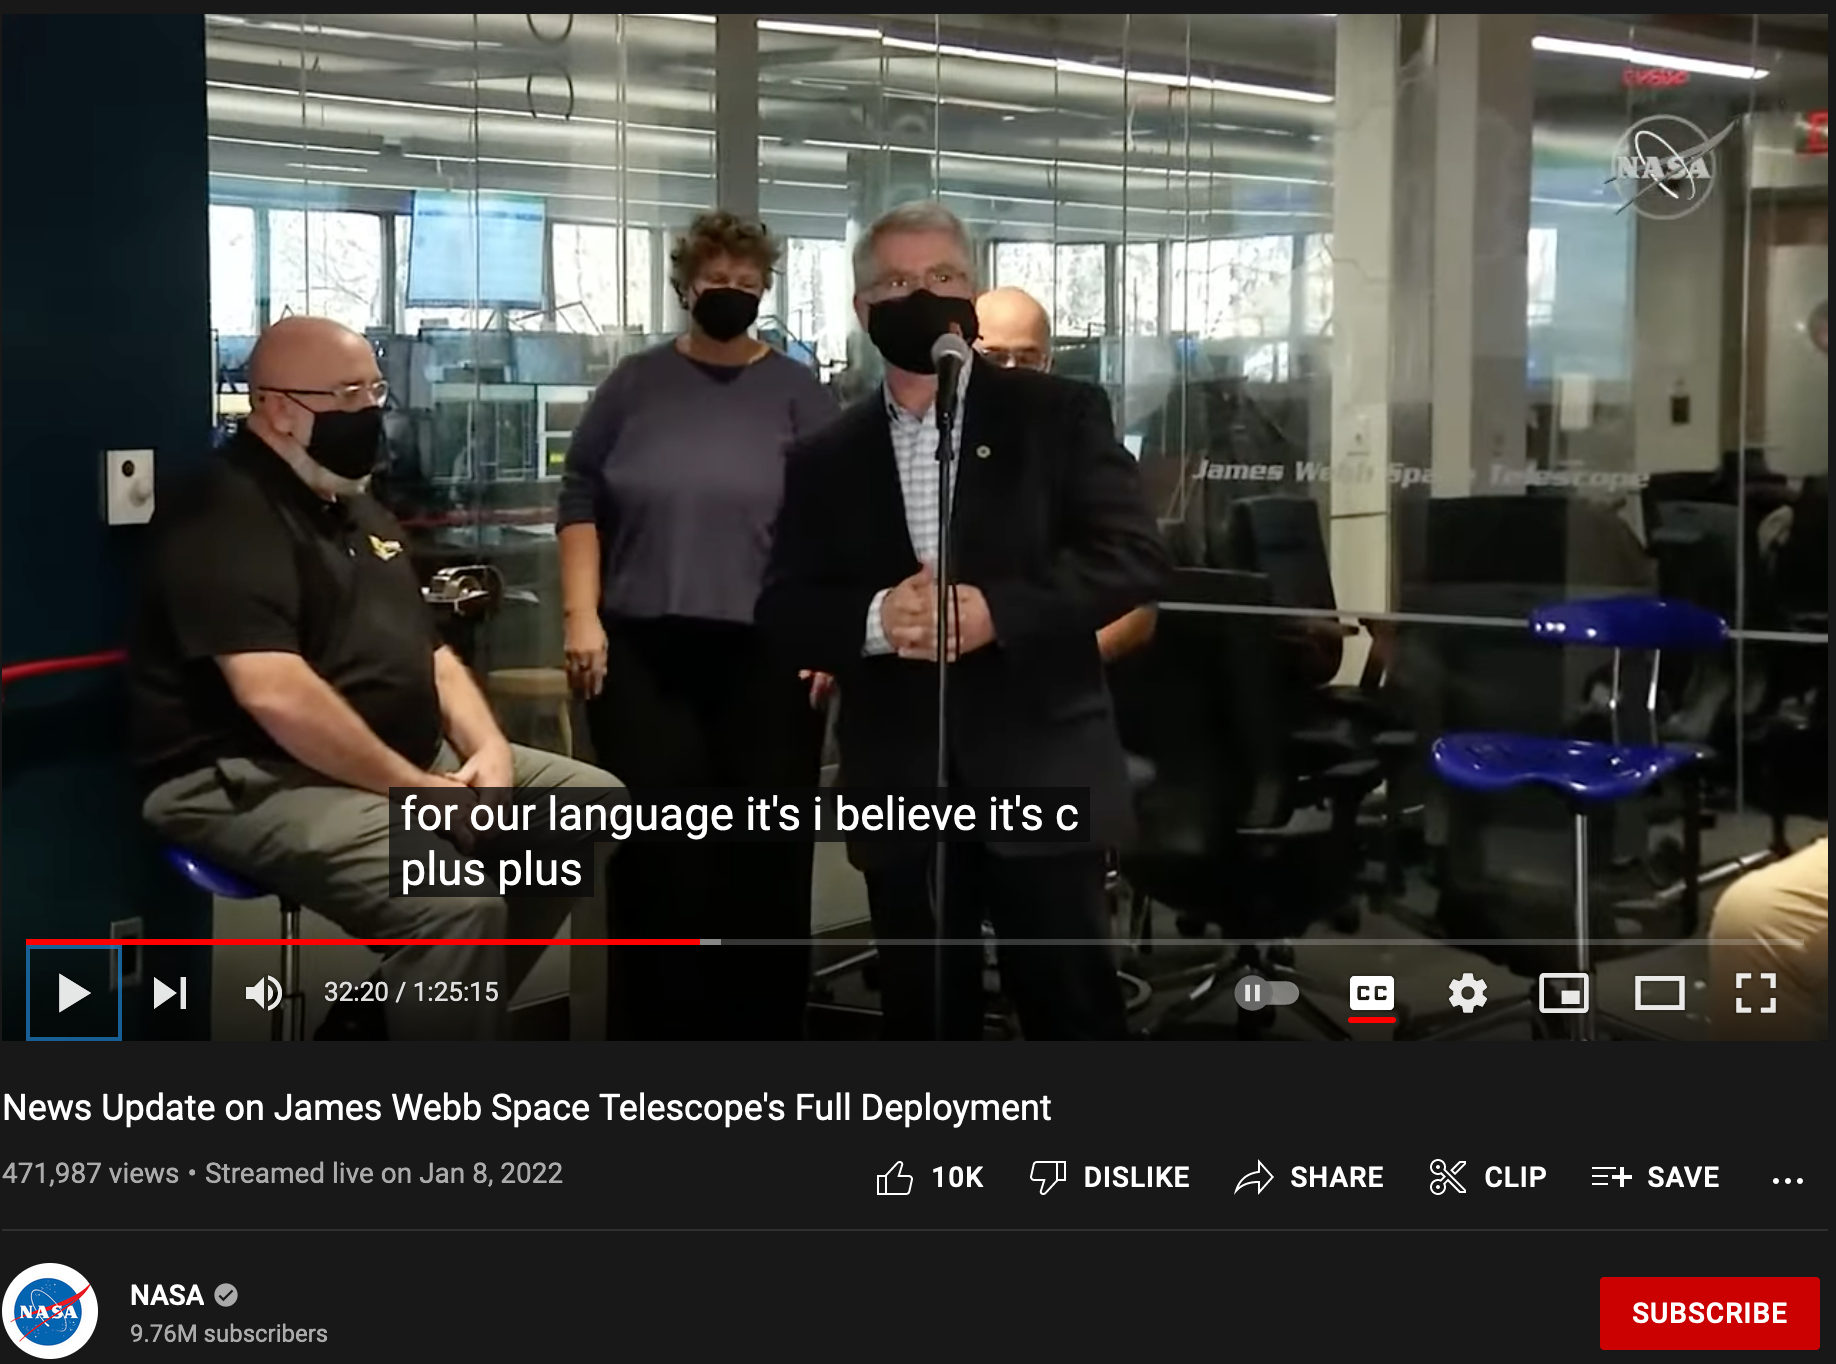
\includegraphics[scale=.1]{webbcpp}
\end{block}

\endinput

\Level 0 {Further reading}

Tutorial, assignments:
\url{http://www.cppforschool.com/}

Problems to practice:
\url{http://www.spoj.com/problems/classical/}
